The rock block generating algorithm is based on a subdivision approach: each discontinuity is introduced sequentially and if it intersects the parent block, the parent block is subdivided into two child blocks. This process is repeated until all discontinuities have been processed and is repeated for each block. \ref{fig:SlicingIllustration} shows a simple schematic of this process. The original serial algorithm is implemented in C++ using data structures to represent the blocks and discontinuities. \par 

\begin{figure}
  \centering
  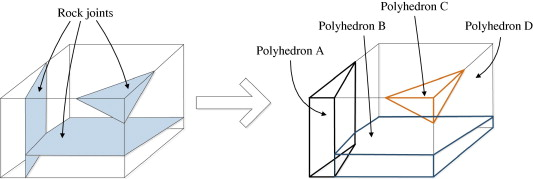
\includegraphics[width=0.75/textwidth]{SlicingIllustration}
  \caption{Polyhedron generation schematic \parencite{Slicing}}
\end{figure}

This algorithm is refactored and modified in Scala to run in parallel on Spark using a functional approach. The following sections give a description of how the different stages of the rock generation process are implemented from a high level. \ref{Details} gives more detail on the actual code generated to do this. 

\subsection{Input Processing}
Before discussing how the input is processed, it is necessary to describe how the rock blocks and discontinueties are represented. The blocks are case classes within Scala that keep a list of faces that define the block as well as the location of its center in global coordinates. The faces are a class themselves that contain the face's normal vector, a distance from the block's origin, as well as the friction angle and cohesion along the face. \par


